% Crucial Preamble
\documentclass[12pt,letterpaper]{article} \usepackage{amsmath} \usepackage{graphicx}  \usepackage{longtable}  \usepackage{amssymb}
%\usepackage[margin=0.7in]{geometry}

\usepackage[left=1.3cm,top=2.5cm,right=1.3cm,bottom=2.5cm,bindingoffset=0cm]{geometry}


% Extra Preamble
\usepackage{fancyhdr} \usepackage{enumitem} \usepackage{float} \usepackage{soul}
\usepackage{multicol} \usepackage[compact]{titlesec}


% frames with display breaks
\usepackage{mdframed}
\allowdisplaybreaks

% change spacing
\usepackage{setspace}
\setlength{\parskip}{0.4\baselineskip}

% Remove paragraph indentation
\setlength{\parindent}{0pt}

% Reduce space before and after section headings
\titlespacing*{\section}{0pt}{0.1\baselineskip}{0.2\baselineskip}

% changes font
%\renewcommand{\familydefault}{\sfdefault}

% adds header and footer
\pagestyle{fancy}
\fancyhead{} \fancyhead[C]{Whole Year Cheat Sheet} \fancyhead[L]{MAT1348} \fancyhead[R]{Owen Daigle}
\fancyfoot{} \fancyfoot[C]{\tiny{PRAISE THE ABSOLUTE}} \fancyfoot[R]{ \thepage }


\begin{document}

    \thispagestyle{empty}
    \begin{center}
        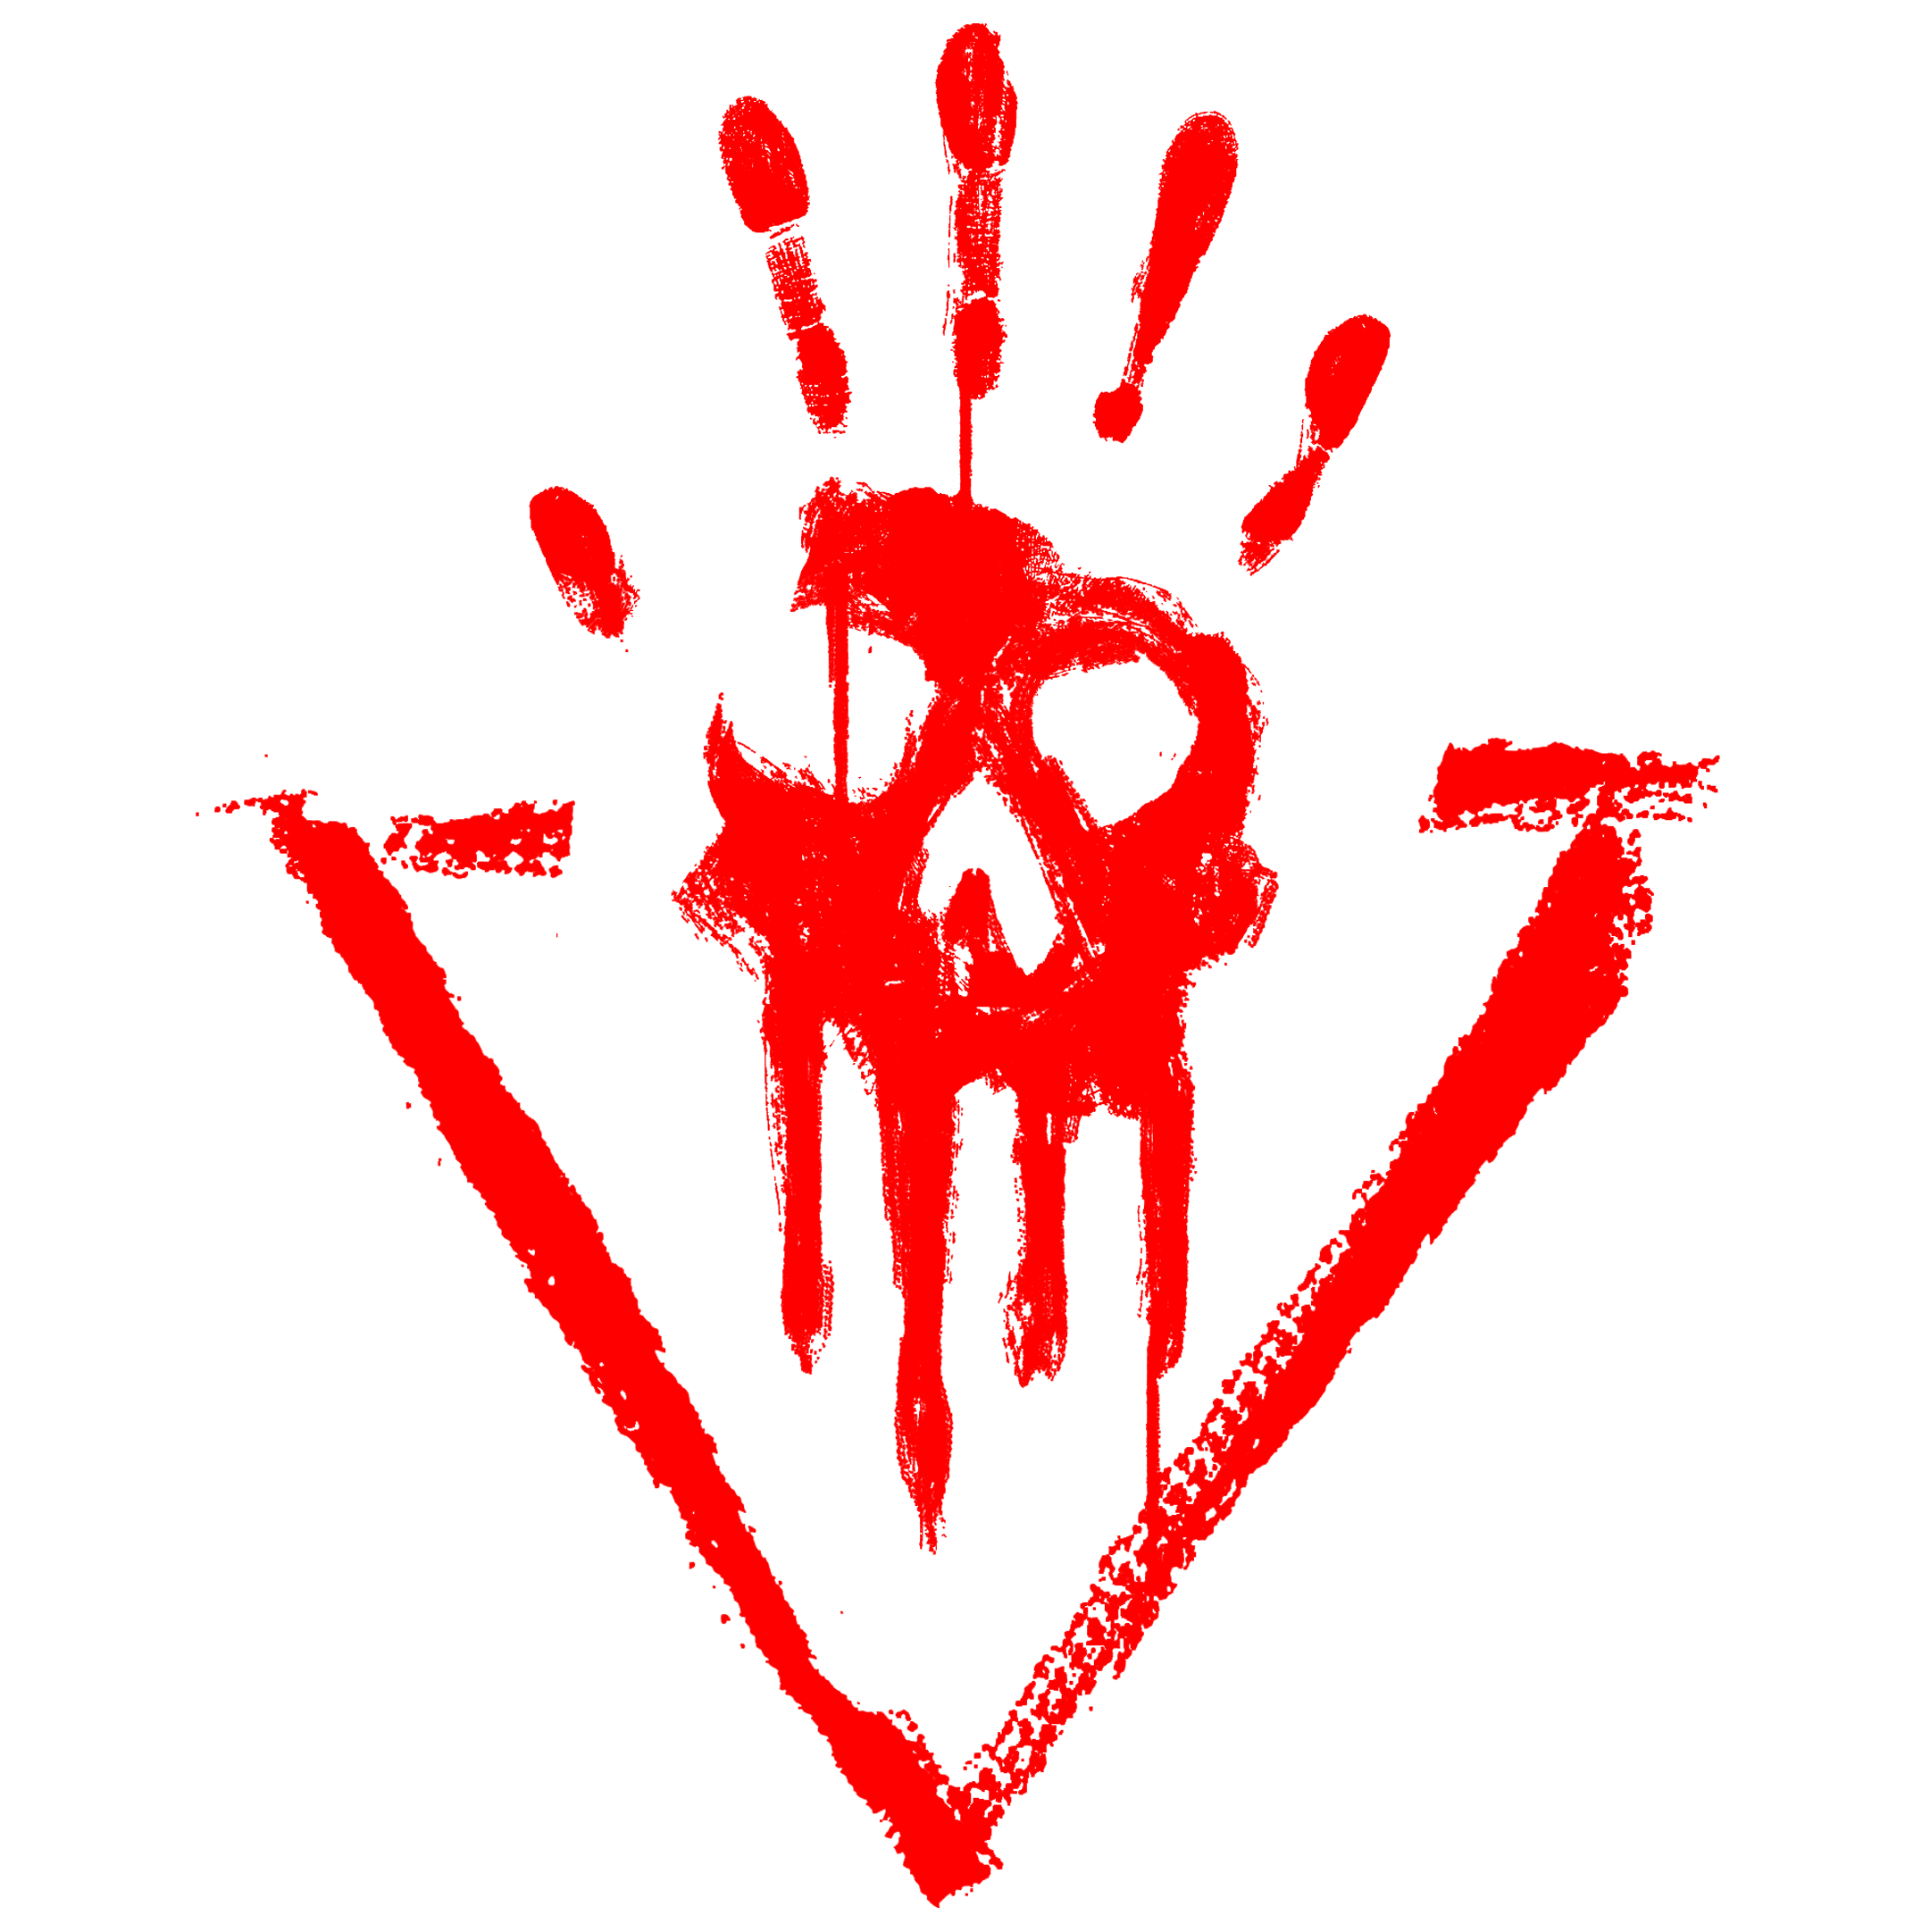
\includegraphics[width=0.12\linewidth]{abs.png}\\
        \vspace{2em}
        \Large\textbf{MAT 1348 Cheat Sheet} \\
        \vspace{0.5em}
        \small{Winter 2024} \\
        \small{University of Ottawa} \\
        \small{Owen Daigle}
    \end{center}

    \pagebreak

    \begin{spacing}{0}
    \tableofcontents
    \end{spacing}

    \pagebreak

    \section{Propositional Logic}

        \subsection{Propositions}
        A proposition is a \emph{declaritave statement} that is \emph{either True or False}.

        \begin{mdframed}
            \textbf{Ex. }
            \begin{itemize}[noitemsep]
                \item $1+1=2$ is a proposition with truth value \textbf{T}
                \item $ 1 + 1 = 0$ is a proposition with truth value \textbf{F}
                \item "I like blueberries" Is a proposition with a truth value \textbf{T}. Note, this depends on who is considered as "I".
                \item $1+x=4$ is not a proposition since we have not defined x. 
                \item "Do you like blueberries" is \emph{not} a proposition since it has no truth value.
            \end{itemize}
        \end{mdframed}

        We assign propositions to variables. 

        \begin{mdframed}
            \textbf{Ex. }Let P represent "I like blueberries"
        \end{mdframed}

        We can find truth tables using propositions. 

        \begin{mdframed}
            \textbf{Ex. } Find the truth table of $(P\rightarrow Q) \leftrightarrow (\lnot P \lor Q)$.

            We create a table with 4 rows, since there are 2 propositions and therefore 4 total combinations. 

            Then we can break up the whole proposition into smaller parts. 

            Finally, we can find the truth values for all the parts. This should be fairly obvious, but if not, more information is provided in the appendix.

            \begin{figure}[H]
                \centering
                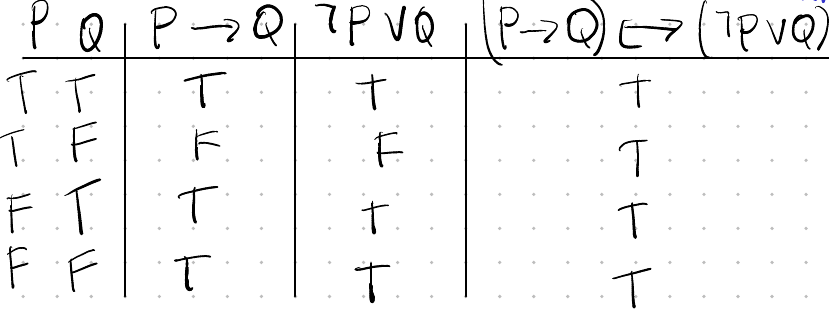
\includegraphics[width=0.5\linewidth]{ex1.png}
            \end{figure}

            This is known as a Tautaulogy since it is always true. If it had been always false, it would have been a contradiction. Otherwise, it would have been a contingency.
        \end{mdframed}

        To convert from regular english to logic, this table helps. 

        \begin{figure}[H]
            \centering
            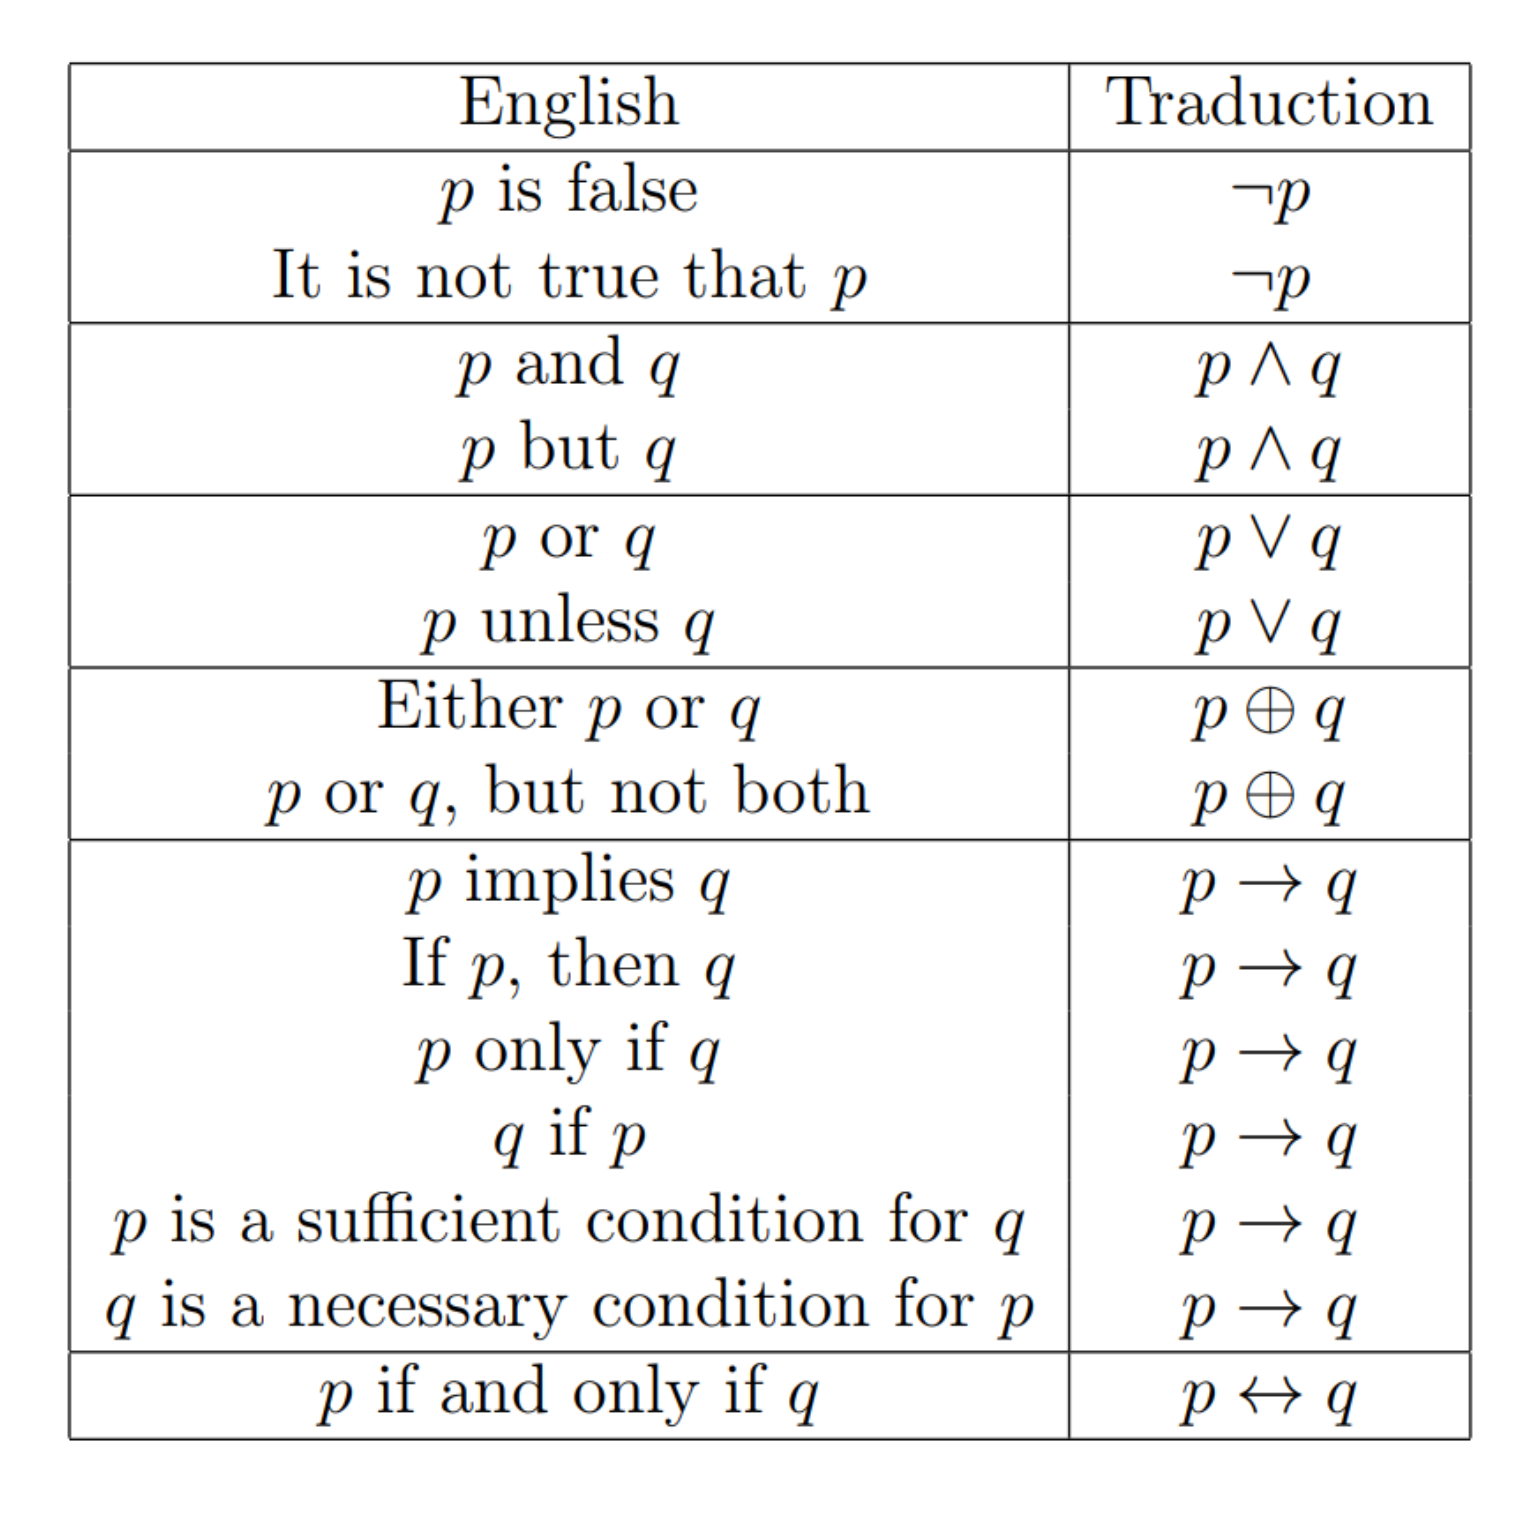
\includegraphics[width=0.5\linewidth]{eng_to_logic.png}
        \end{figure}

        \subsection{Normal Forms}
        The \emph{Disjunctive Normal Form} of a propositional statement are all the combinations of propositions that make the statement true (using And) all connected together using Or. 
        
        The \emph{Conjunctive Normal Form} of a propositional statement is similar to the DNF form, except it is the combination of all propositions that make it false (using Or) all connected together using And. 

        \begin{mdframed}
            \textbf{Ex. } Find the CNF and DNF of $P \oplus Q$.

            First we create the truth table. 

            \begin{figure}[H]
                \centering
                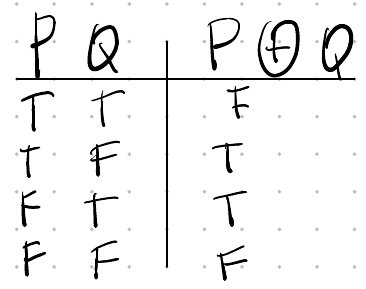
\includegraphics[width=0.2\linewidth]{ex2.png}
            \end{figure}

            For DNF, we look wherever it is true. We see 2 rows. 

            Then we take those 2 rows (where Q and P are connected using And) and connect it using Or. 
            \begin{align*}
                P\oplus Q \equiv (P\land \lnot Q) \lor (\lnot P \land Q)
            \end{align*}

            For the CNF, we do the opposite (using rows that are false).
            \begin{align*}
                P\oplus Q \equiv (P\lor Q) \land (\lnot P \lor \lnot Q)
            \end{align*}
    
        \end{mdframed}

        \subsection{Knights and Knaves}
        Knights \emph{always} tell the truth, and Knaves \emph{always} lie. In these examples, we need to find out who is a knight, and who is a knave. 

        \begin{mdframed}
            \textbf{Ex. } We have the following situation involving 3 Knights and Knaves, A, B, and C.

            A says: "We are all knaves"
            
            B says: "Exactly one of us is a knight"

            C says nothing.

            What are the identities of A, B, and C?

            To solve this, we create a truth table. We let a, b, c, represent whether A, B, C respectively are knights (T), or knaves (F).

            \begin{centering}
                \begin{tabular}{c c c|c|c}
                    \textbf{$a$} & \textbf{$b$} & \textbf{$c$} & \textbf{A says} & \textbf{B says} \\
                    \hline
                    T & T & T & F & F\\
                    T & T & F & F & F\\
                    T & F & T & F & F\\
                    T & F & F & F & T\\
                    F & T & T & F & F\\
                    F & T & F & F & T\\
                    F & F & T & F & T\\
                    F & F & F & T & F\\
                \end{tabular}

            \end{centering}

            We fill the 4th and 5th column with whether what A said was true, and whether what B said was true according to their identities in the first 3 columns. 

            For example, in the first column, A is speaking falsely since in that situation they are all knights, not knaves like A said. B is also speaking falsely since more than one person is a knight. 

            Then, we need to align what they are saying with what they are. So in row 1, we see that A is a knight (column 1) and A is lying (column 4). This is impossible. B is also a knight (col 2) and they are also lying (col 5).

            We do this for all the rows and end up finding out that the only row that makes sense, is the 6th row where B is the only knight. This is because A is both lying and a knave, and B is  both telling the truth and a knight. 

        \end{mdframed}

        With these problems, if there are no plausible situations, then this situation cannot exist. 

        If there are multiple plausible solutions, then we cannot know the identities of the individuals. 

        \subsection{Logic Laws}
        There are 23 logic laws. These are found in the appendix. These laws can be used to prove that 2 statements are equivalent by manipulating one statement to resemble the other. 

        \subsection{Truth Trees}
        As the number of propositions increases, truth tables get exponentially bigger. Truth trees are another way of representing propositions which do not get as big. 

        For each proposition in a compound proposition, we create a branch of the tree. 
        
        When we finish with \emph{all} propositions, we go up each path and check if there are any contradictions. If there are, we kill that path.

        If there are no remaining paths, then the root is a contradiction.

        These are the rules we use. 
        \begin{figure}[H]
            \centering
            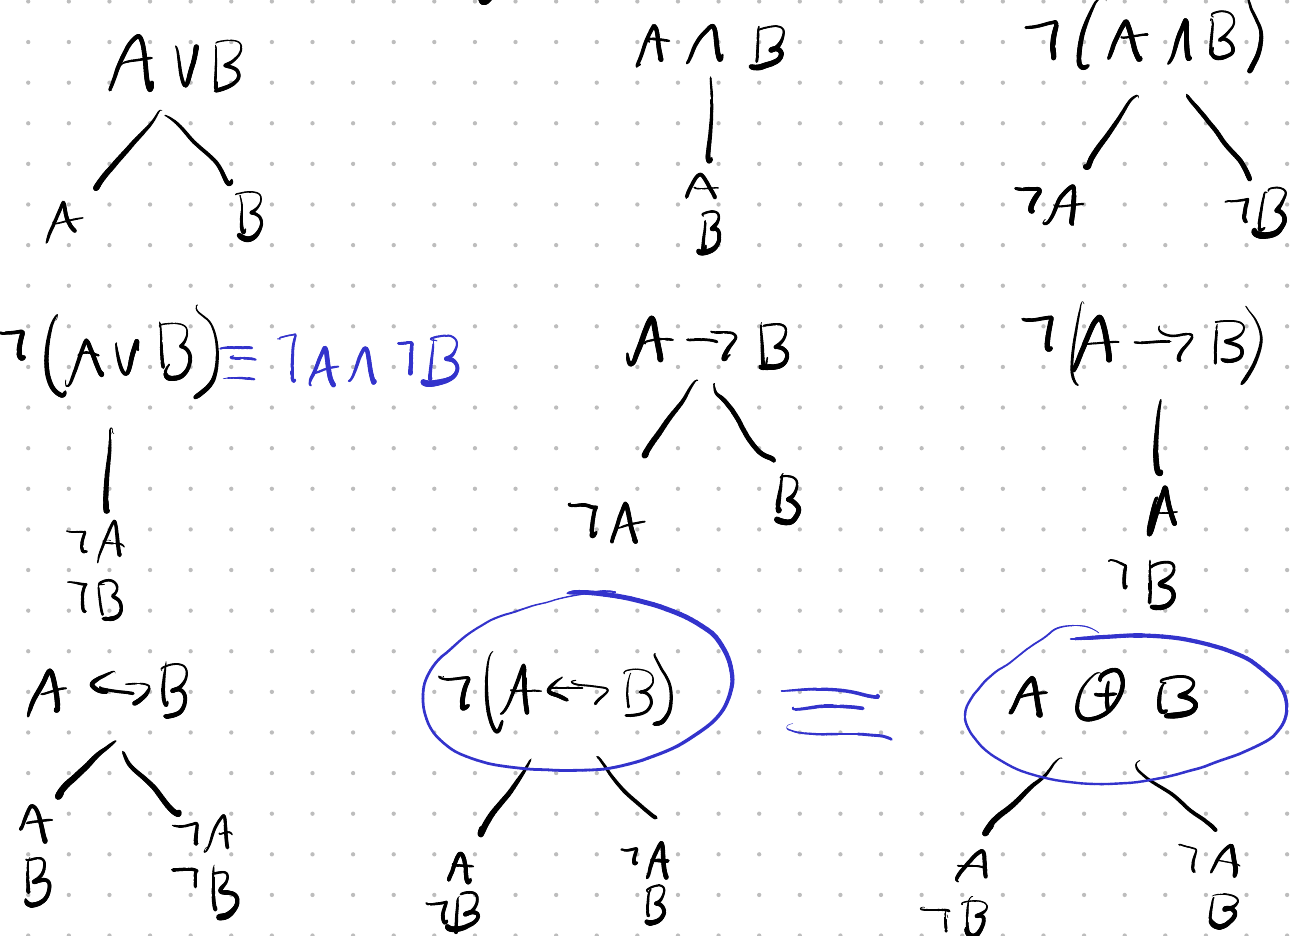
\includegraphics[width=0.8\linewidth]{truth_tree.png}
        \end{figure}

        \begin{mdframed}
            \textbf{Ex. } Is the following compound proposition a tautaulogy?
            \begin{align*}
                \lnot(\lnot B \rightarrow (A \lor C))\lor ((\lnot A \land \lnot B)\rightarrow C)
            \end{align*}

            This would not be too bad to do with a truth table, but still easier with a truth tree.

            The trees do not help us with tautaulogies, but they can show if something is a contradiction. So, if the negation of our compound proposition is a contradiction, then the original compound proposition \emph{must} be a tautology. 

            \begin{figure}[H]
                \centering
                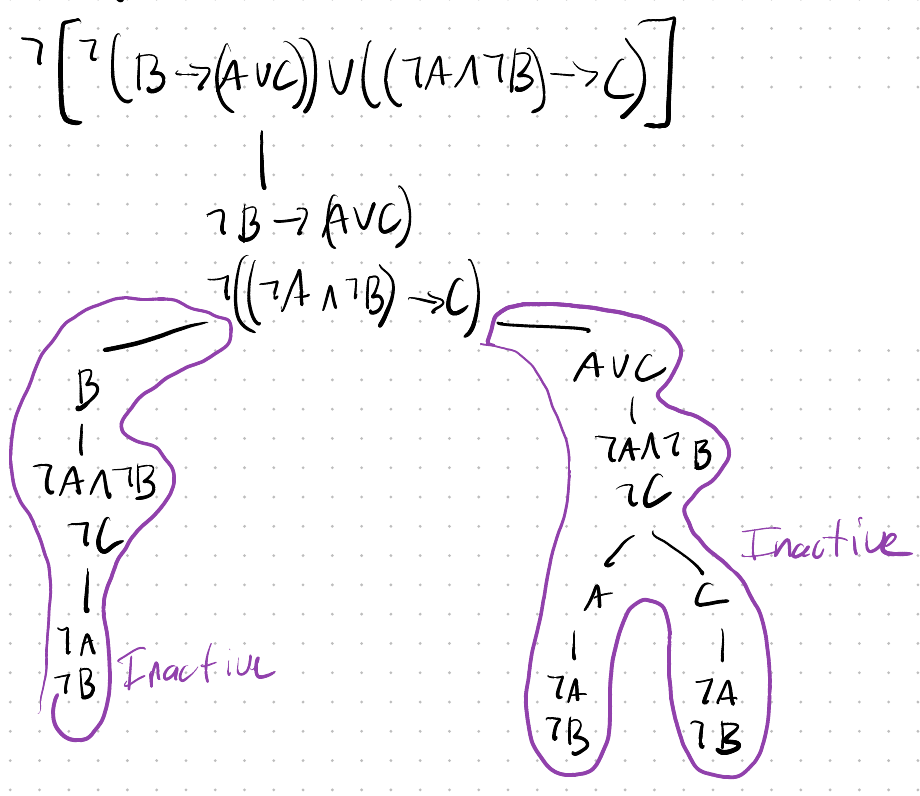
\includegraphics[width=0.7\linewidth]{ex3.png}
            \end{figure}

            Since there are no active roots (each root has a contradiction such as $A$ and $\lnot A$), then the root is a contradiction and therefore the original expression is a tautology.
        \end{mdframed}

        \subsection{Logical Equivalences}
        2 propositions $P$ and $Q$ are logically equivalent ($P \equiv Q$) iff $P\leftrightarrow Q$ is a tautology.

        So we can prove 2 statements $P$ and $Q$ are logically equivalent by making the truth tree of $\lnot (P \leftrightarrow Q)$. If it is a contradiction (no active paths), then they are logically equivalent. If there is an active path, then they are not logically equivalent. 

        \subsection{Arguments}
        An argument is a type of proposition. It has the form of: 
        \begin{align*}
            P_1 \land P_2 \land ... \land P_k \rightarrow C
        \end{align*}

        where $P_1 \land P_2 \land ... \land P_k$ is the hypothesis, and $C$ is the conclusion. 

        $P_1 \land P_2 \land ... \land P_k \rightarrow C$ is valid if it is a tautology. 

        An example can be found in the appendix.

    \section{Proofs}

        \subsection{Direct Proof ($P \rightarrow Q$)}
        In direct proofs, we assume $P$, and then show $Q$. 

        \begin{mdframed}
            \textbf{Ex. } Prove that if $n$ is odd, then $n^2$ is odd.

            To do this, we need the definition of an odd number. 

            \begin{centering}
                \fbox{\parbox{5.5in}{An integer $n$ is even if $\exists$ an integer $k$ such that $n=2k$}}

                \fbox{\parbox{5.5in}{An integer $n$ is odd if $\exists$ an integer $k$ such that $n=2k+1$}}

            \end{centering}

            We let $P = $ "n is odd", and $Q = $ "$n^2$ is even".

            Using a direct proof, we show that if $P$, then $Q$. 

            Suppose $n$ is odd, then $\exists \text{ } k\in\mathbb{Z}$ such that $n=2k+1$. Then:
            \begin{align*}
                n^2 = (2k+1)^2 = 4k^2 + 4k + 1 = 2(2k^2+2k)+1
            \end{align*}

            This looks just like the definition of an odd number.

            Since $k\in\mathbb{Z}$, then so is $2k^2+2k$.

            Therefore, $\exists \text{ } m\in\mathbb{Z}$ such that $n^2=2m+1$, therefore $n^2$ is odd.
        \end{mdframed}

        \subsection{Indirect Proof ($P \rightarrow Q$)}
        Here, we assume $Q$ is false, and then show that $P$ must also be false.

        \begin{mdframed}
            \textbf{Ex. } Prove that if $5n+4$ is odd, then $n$ is odd.

            We let $P = $ "$5n+4$ is odd", and $Q=$ "$n$ is odd".

            We assume that $n$ is even, and show that $5n+4$ must therefore also be even.

            Suppose $n$ is an even integer, $\exists \text{ } k\in\mathbb{Z}$ such that $n=2k$.
            \begin{align*}
                5n+4 = 5(2k)+4 = 10k+4 = 2(5k+2)
            \end{align*}

            This looks just like the definition of an even number.

            Since $k\in\mathbb{Z}$, so is $2(5k+2)$.

            So $\exists \text{ } m\in\mathbb{Z}$ such that $5n+4=2m$, therefore $5n+4$ is even.

            Since we proved the $\lnot Q \rightarrow \lnot P$, then therefore $P\rightarrow Q$.
        \end{mdframed}

        \subsection{Contradiction ($P \rightarrow Q$)}
        Here we assume that $P$ is true, and $Q$ is false, and then find a contradiction. 

        This contradiction can be something like $2=1$, or something a bit less obvious like $1=3(3k+3k^2), k\in\mathbb{Z}$. Here 1 \emph{cannot} be the product of 3, and an integer. 

        \begin{mdframed}
            \textbf{Ex. } Let $n\in \mathbb{Z}$. Show that if $n^2+5$ is odd, then $n$ is even. 

            We will assume $n^2+5$ is odd, and $n$ is also odd, and then find a contradiction. 

            This means that $n^2 + 5 = 2k+1, k\in\mathbb{Z}$, and $n^2 = 2m+1, m\in\mathbb{Z}$.
            \begin{align*}
                &n^2 + 5 = 2k+1 \\
                &\implies 5 = 2k+1-n^2 = 2k+1-(2m+1)^2 = 2k+1-4m^2-4m-1 = 2k-4m^2-4m\\
                &= 2(k-2m^2-2m)
            \end{align*}
            This is saying that $5=2(k-2m-2m^2)$ which implies 5 is even. This is a contradiction. 

            Since $P\rightarrow \lnot Q$ is a contradiction, then $P\rightarrow Q$ is true. 
        \end{mdframed}

        \subsection{Proof by Case ($P \rightarrow Q$)}
        This is where we break up a problem into multiple cases, and then prove each case using other methods. 

        \subsection{Empty Proof ($P \rightarrow Q$)}
        If we can show that $P$ is always false, then we know that $P \rightarrow Q$ is always true. 

        \subsection{Trivial Proof}
        If we show that $Q$ is always true, then we know that $P \rightarrow Q$.

    \section{Set Theory}
    A set is a collection of objects called elements. 

    For example, the set A with numbers 1, 2, and 3 is denoted $A=\{1,2,3\}$

        \subsection{Empty Set}
        The empty set denoted $\emptyset$ is the set that contains no elements. 
        \begin{align*}
            x\in\emptyset \text{ is false } \forall \text{ }x
        \end{align*}

        \subsection{Subsets}
        Let $A$ and $B$ be 2 sets. We say $A$ is a subset of $B$ if all elements in $A$ are also in $B$, denoted $A\subseteq B$.

        \begin{mdframed}
            \textbf{Ex. } We have 3 sets, $A=\{a,b,c\}, B=\{a,c\}, C=\{a,\{B\},c\}$.

            We can say:
            
            $B\subseteq A$ is True

            $B\subseteq C$ is True

            $A\subseteq B$ is False since $b\in A, b\notin B$

            $C\subseteq A$ is False since $\{b\} \in C, \{b\} \notin A$. Note that $b\ne \{b\}$.

            $A\subseteq A$ is True

            $\emptyset \subseteq A$ is True
        \end{mdframed}

        \subsection{Proper Subset}
        Suppose we have 2 sets $A$, and $B$. We say $A$ is a proper subset of $B$ denoted $A\subset B$ if:
        \begin{itemize}[noitemsep]
            \item $A\subseteq B$
            \item $A\ne B$
        \end{itemize}

        \subsection{Cardinality}
        Cardinality is just the number of distinct elements in a set $A$ denoted $|A|$. 

        \begin{mdframed}
            \textbf{Ex.} These are the cardinalities of some sets.
            \begin{align*}
                |\{a,b,c\}| = 3\\
                |\{a,a,a,a,a,a,b,c,c\}| = 3\\
                |\{a,\{a\},\{a,\{a,\{a\}\}\}\}| = 3\\
                |\emptyset| = 0\\
                |\{\emptyset\}| = 1
            \end{align*}

        \end{mdframed}

        \subsection{Power Set}
        The power set of a set $A$ is the set of all subsets of $A$. 

        \begin{mdframed}
            \textbf{Ex. } Find the power set of $A = \{a,b,c\}$.
            \begin{align*}
                P(A) = \{\emptyset, \{a\}, \{b\}, \{c\}, \{a,b\}, \{a,c\}, \{b,c\}, \{a,b,c\}\}
            \end{align*}

            Note that we include all sets \emph{including} the empty set. 

            
        \end{mdframed}

        We see that if $|A| = n \implies |P(A)| = 2^n$.

        \subsection{Cartesian Product}
        \begin{mdframed}
            \textbf{Ex. } Let $A=\{a,b,c\}, B=\{1,2\}$. Find $A\times B$, and $B\times A$.

            To do this, we will take each element of set $A$, and pair it with each element from the set $B$. Note that for $A\times B$, $A$ is the first half of each pair, and for $B\times A$, $A$ is the second half of each pair. 
            \begin{align*}
                A\times B = \{(a,1), (a,2), (b,1), (b,2), (c,1), (c,2)\}\\
                B\times A = \{(1,a), (1,b), (1,c), (2,a), (2,b), (2,c)\}
            \end{align*}
        \end{mdframed}

        The cardinality of $|A\times B| = |A|\cdot |B|$.

        \subsection{Operations on Sets}

            \subsubsection{Union (or)}
            The union of 2 sets $A$ and $B$ is:
            \begin{align*}
                A\cup B = \{x | x\in A \text{ or } x\in B\}
            \end{align*}

            \begin{figure}[H]
                \centering
                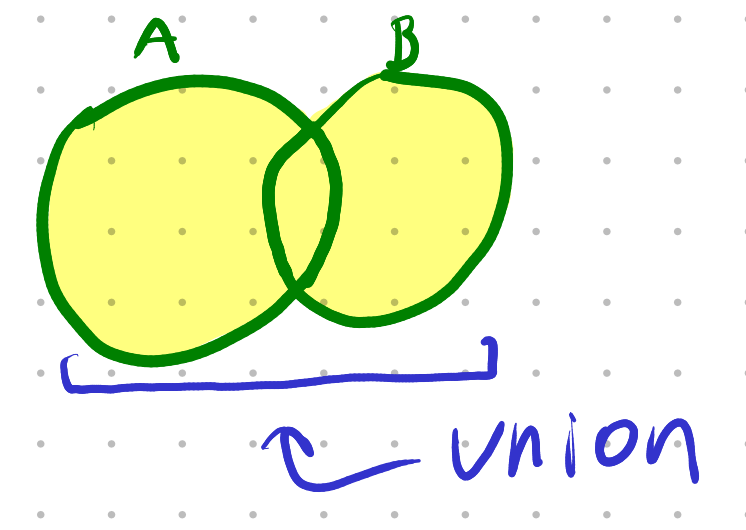
\includegraphics[width=0.3\linewidth]{union.png}
            \end{figure}
            
            \subsubsection{Intersection (and)}
            The intersection of 2 sets $A$ and $B$ is:
            \begin{align*}
                A\cap B = \{x | x\in A \text{ and } x \in B\}
            \end{align*}

            \begin{figure}[H]
                \centering
                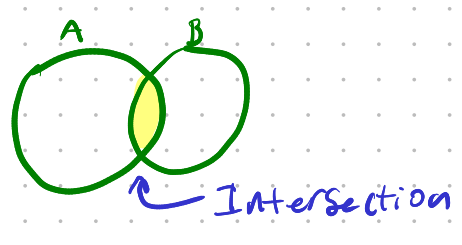
\includegraphics[width=0.3\linewidth]{intersection.png}
            \end{figure}

            \subsubsection{Compliment (not)}
            The compliment of $A$ is: 
            \begin{align*}
                \overline{A} = \{x | x\in U \land x \notin A\}
            \end{align*}
            Where $U$ is the universal set (set of numbers we are currently working with)

            \begin{figure}[H]
                \centering
                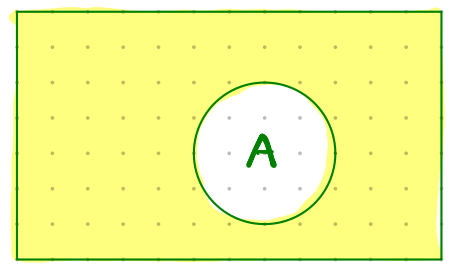
\includegraphics[width=0.3\linewidth]{compliment.png}
            \end{figure}

            \subsubsection{Difference}
            The difference of 2 sets $A$, and $B$ is:
            \begin{align*}
                A-B = \{x | x\in A \land x \notin B\}
            \end{align*}

            \begin{figure}[H]
                \centering
                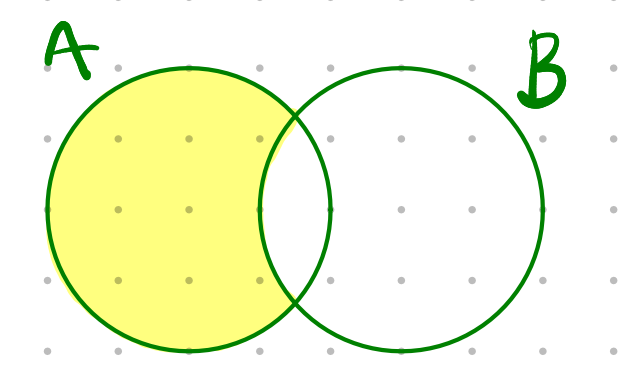
\includegraphics[width=0.3\linewidth]{difference.png}
            \end{figure}

            \subsubsection{Symmetric Difference (xor)}
            The symmetric difference of $A$ and $B$ is:
            \begin{align*}
                A \oplus B = \{x | x\in A \oplus x \in B\}
            \end{align*}

            \begin{figure}[H]
                \centering
                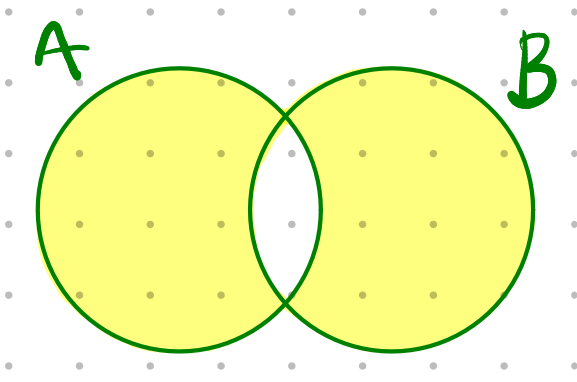
\includegraphics[width=0.3\linewidth]{symmetric_diff.png}
            \end{figure}

        \subsection{Set Identities}
        A set identity is an equation that is true no matter the sets considered. 

        They are very similar to the laws of logic, except there are a few added for \emph{set differences}. 
        \begin{align*}
            A-B=A\cap \overline{B}\\
            A\oplus B = (A-B) \cup (B-A)\\
            A\oplus B = (A\cup B) - (A\cap B)
        \end{align*}

        Because of this similarity between propositional logic and set logic, we can also solve set problems using tables. However we do not call them truth tables, but rather \emph{Membership Tables}.

        \begin{mdframed}
            \textbf{Ex. } Show using a membership table that $\overline{B\cup C - A} = (\overline{C}\cap \overline{B})\cup A$.
            \begin{figure}[H]
                \centering
                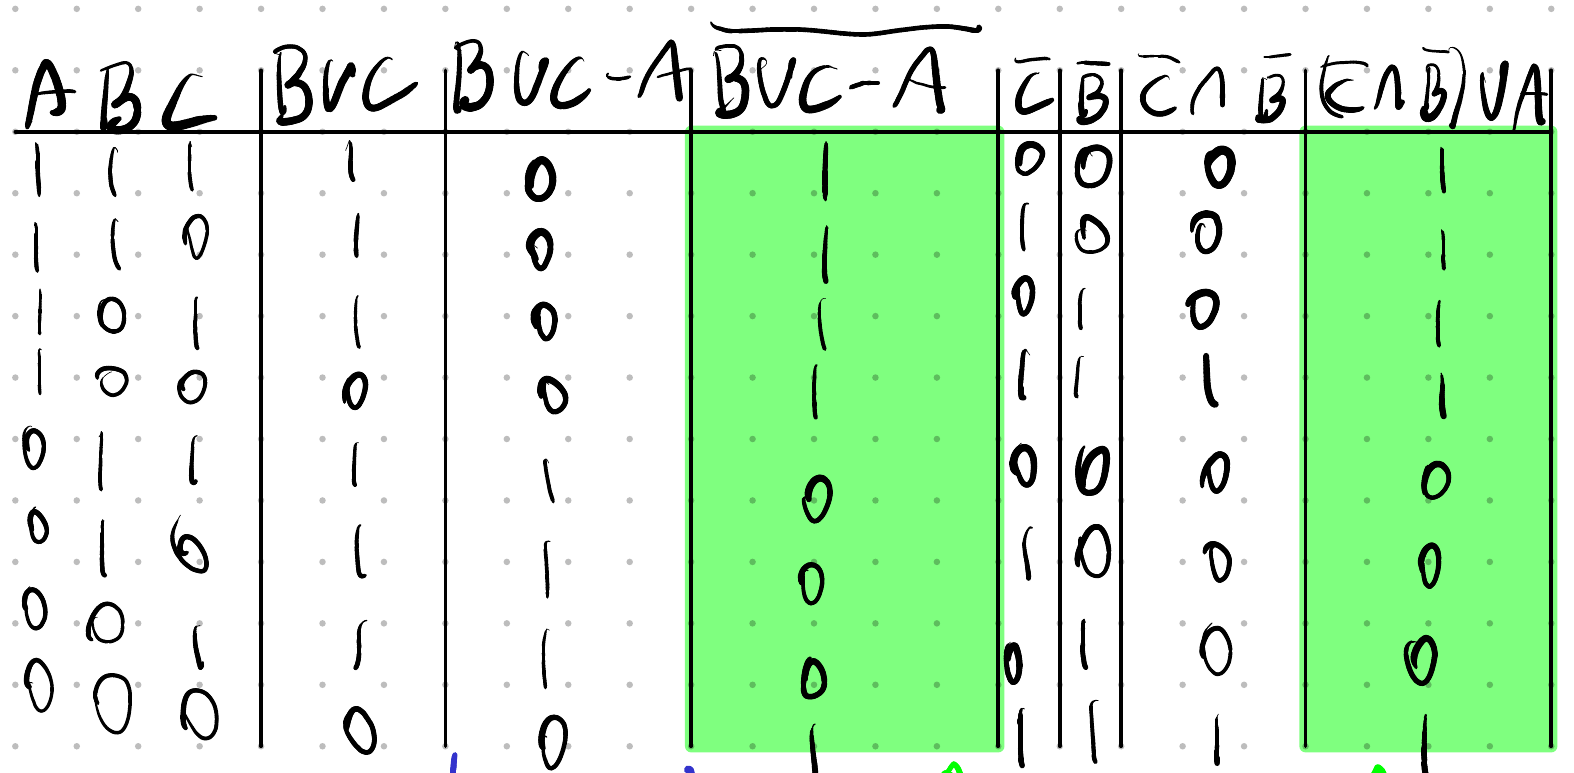
\includegraphics[width=0.6\linewidth]{ex5.png}
            \end{figure}
            We see that the two columns corresponding to each side of the set equation are equivalent, therefore it is proven.
        \end{mdframed}

    \section{Relations}

        \subsection{Types of Relations}

            \subsubsection{Reflexive}
            A relation $R$ on a set $A$ is reflexive if $\forall \text{ }x$, $x$ is related to $x$.

            \subsubsection{Symmetric}
            A relation $R$ on a set $A$ is symmetric if $\forall \text{ } x, y \in A$:
            \begin{align*}
                (x,y)\in R \to (y,x) \in R
            \end{align*}

            \subsubsection{Antisymmetric}
            A relation $R$ on a set $A$ is antisymmetric if $\forall \text{ } x,y \in A$:
            \begin{align*}
                (x,y)\land (y,x) \to x=y
            \end{align*}

            \subsubsection{Transitive}
            A relation $R$ on a set $A$ is transitive if $\forall \text{ }x,y,z \in A$:
            \begin{align*}
                (x,y)\in R \land (y,z)\in R \to (x,z)\in R
            \end{align*}

        \subsection{Equivalence Relation}
        A relation $R$ is an Equivalence Relation if it is reflexive, symmetric, and transitive. 

        \begin{mdframed}
            \textbf{Ex.} Prove the following relation is an equivalence relation:
            \begin{align*}
                (a,b)\in R \leftrightarrow a-b \text{ is even}
            \end{align*}
            We need to prove that is is reflexive, symmetric, and transitive. 

            Once those 3 things are proven, then we know that it must be an equivalence relation. 

            \begin{figure}[H]
                \centering
                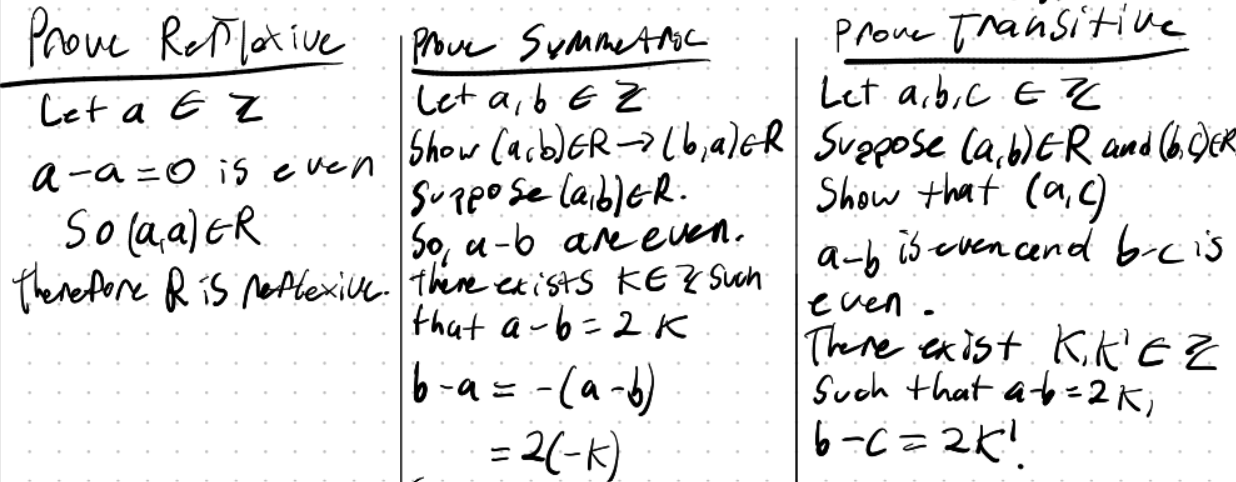
\includegraphics[width=0.9\linewidth]{prove-equi-1.png}
            \end{figure}

            \begin{figure}[H]
                \centering
                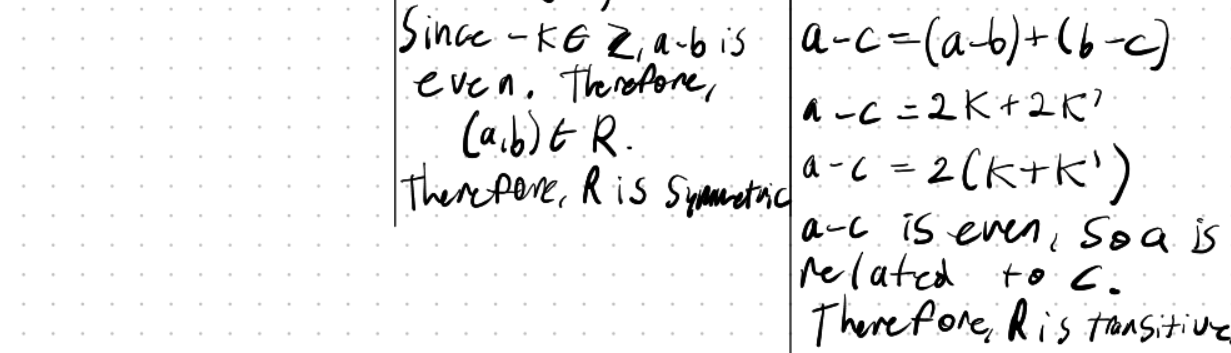
\includegraphics[width=0.9\linewidth]{prove-equi-2.png}
            \end{figure}

        \end{mdframed}

        \subsection{Counting Relations}
        The number of relations from a set $A$ to another set $B$ is $|P(A\times B)| = 2^{|A\times B|} = 2^{|A|\cdot|B|}$

        \subsection{Visually Representing Relations}
        To visually represent a relation with points in the form of $(x,y)$, we draw a point for each element of the relation. 

        Then for each pair, we draw an arrow going from the point corresponding to $x$, to the point corresponding to $y$. 

        Once we have done that for all elements in the relation, we can get the four properties using the following rules. 
        \begin{itemize}[noitemsep]
            \item The relation is reflexive if \emph{each} vertex has a loop.
            \item The relation is symmetric if \emph{wherever} there is an arrow, there \emph{is the opposite arrow}. 
            \item The relation is antisymmetric if \emph{whenever} there is an arrow, there is \emph{no opposite arrow}.
            \item The relation is transitive if \emph{every} 2 step path can be done in one step. 
        \end{itemize}

        \begin{mdframed}
            Show the following relation $R$ visually, and check what properties the relation has.
            \begin{align*}
                R = \{(1,1), (2,2), (2,3), (3,2), (3,4)\}
            \end{align*}   
            
            We go ahead and draw the arrows corresponding to each pair of numbers. 

            \begin{figure}[H]
                \centering
                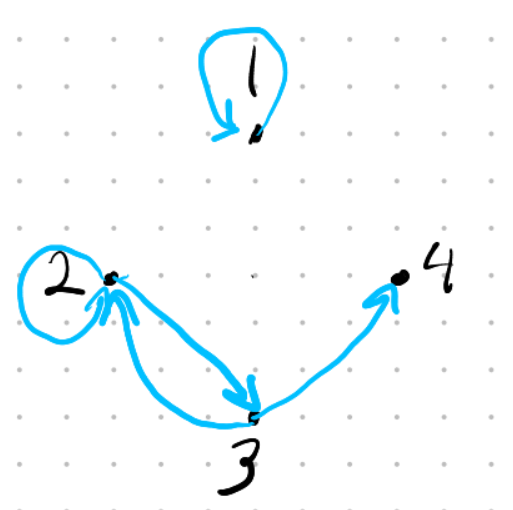
\includegraphics[width=0.2\linewidth]{related_visual.png}
            \end{figure}

            We see that this relation has none of the 4 properties. 
            \begin{itemize}[noitemsep]
                \item Not reflexive since 3 is not related to 3, and 4 is not related to 4.
                \item Not symmetric because 3 is related to 4, but 4 is not related to 3. 
                \item Not antisymmetric since 2 is related to 3, and 3 is related to 2, but 3 $\ne$ 2. 
                \item Not transitive since 2 is related to 3, and 3 is related to 4, but 2 is not related to 4. 
            \end{itemize}
            
        \end{mdframed}

        \subsection{Equivalence Classes}
        Let $R$ be an \emph{equivalence relation} on $A$. Let $a\in A$. The equivalence of $a$ is:
        \begin{align*}
            [a]_R = \{x\in A | aRx\}
        \end{align*}

        \begin{mdframed}
            \textbf{Ex. } Find the equivalence classes for the following relation:
            \begin{figure}[H]
                \centering
                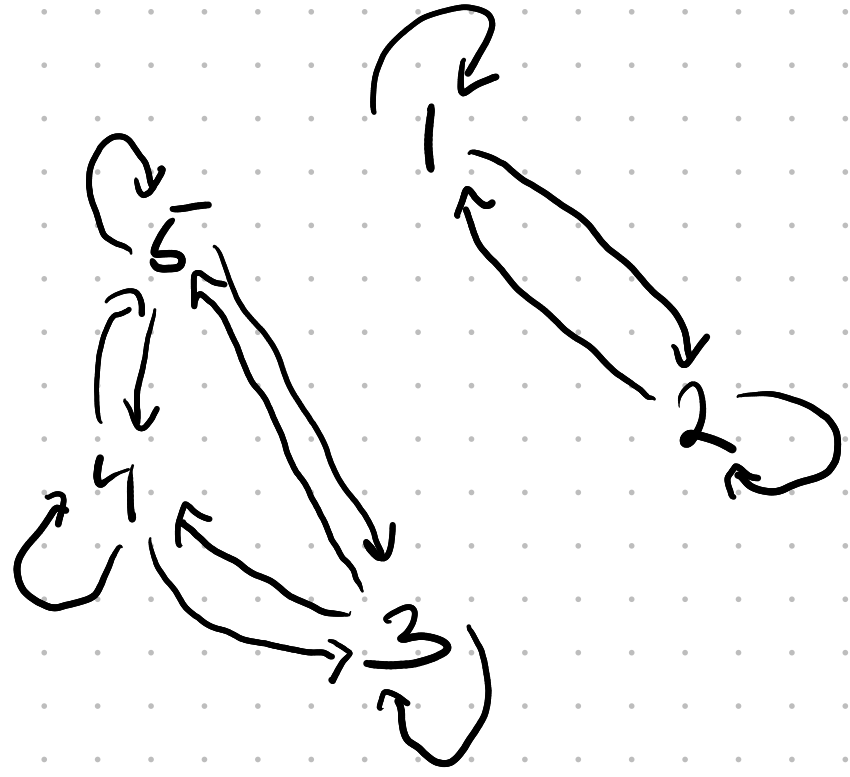
\includegraphics[width=0.25\linewidth]{ex6.png}
            \end{figure}
            \begin{align*}
                &[1]=\{1,2\} = [2] = \{1,2\} &[3] = \{3,4,5\} = [4]=[5]
            \end{align*}
            We see that each "group" is all in the same equivalence class. 
        \end{mdframed}

        \subsection{Modular Arithmetic}
        Let $a\in \mathbb{Z}, m\in \mathbb{N}$.

        We define "$a$ mod $m$" to be the remainder of the division of $a$ by $m$.

        $m$ is called the modulus.

        If $a$ mod $m$ $= b$ mod $m$, then $a$ is congruent to $b$ mod $m$.

        \begin{mdframed}
            \textbf{Ex.} Compute $a$ mod $4$ for each of element of $A$.
            \begin{align*}
                A = \{-100, -10, -4, -3, -2, -1, 0, 1, 2, 3, 4, 11\}
            \end{align*}

            This means compute the closest divisible number that is smaller than $a$.

            $-100$ mod $4$ = $0$\\
            $-10$ mod $4$ = $2$\\
            $-4$ mod $4$ = $0$\\
            $-3$ mod $4$ = $1$\\
            $-2$ mod $4$ = $2$\\
            $-1$ mod $4$ = $3$\\
            $0$ mod $4$ = $0$\\
            $1$ mod $4$ = $1$
        \end{mdframed}

        \subsection{Partitions}
        A partition of $A$ is a set $D=\{p_1,p_2,...\}$ of subsets of $A$ such that:
        \begin{itemize}[noitemsep]
            \item $p_i \ne \emptyset \forall \text{ } i$
            \item $A = p_1 \cup p_2 \cup ...$
            \item $p_i \cap p_j = \emptyset \text{ if } i\ne j$
        \end{itemize}

        \begin{mdframed}
            \textbf{Ex. } Which of these are partitions of $A$.
            \begin{align*}
                A = \{1,2,3,4,5\}
            \end{align*}

            \begin{enumerate}
                \item \{\{3,4,1\},\{2\},\{5\}\}
                \item \{\{3,4,1\},\{1,2,5\}\}
                \item \{\{1\},\{3,4,5\}\}
                \item \{\{1,2,3,4,5\},\{\}\}
            \end{enumerate}

            Only $1.$ is a partition of $A$.

            $2.$ is not a partition since the element $1$ is repeated. $3.$ is not a partition since the element $2$ is excluded. $3.$ is not a partition since one part is the empty set. 
        \end{mdframed}

    \section{Functions}
    A function is a way to assign an element of one set to each element of another set. 
    
    A function has a domain and a codomain. \emph{Each} element in the domain must be assigned to \emph{exactly} one item in the codomain. 

        \subsection{Injective Functions}
        A function $f:A\rightarrow B$ is injective for all $x,y \in A$ if $f(x)=f(y) \rightarrow x=y$.

        This is basically saying that each input has \emph{exactly} one output. 2 different inputs \emph{must} have 2 different outputs. 
        
        We can reason that if $f: A\rightarrow B$, and $A$ is injective, than $|A| \le |B|$.

        \begin{figure}[H]
            \centering
            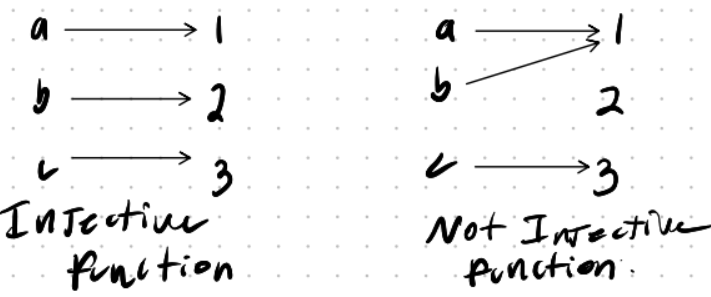
\includegraphics[width=0.5\linewidth]{injective.png}
        \end{figure}

        \begin{mdframed}
            \textbf{Ex. } $f: \mathbb{R} \rightarrow \mathbb{R}, f(x)=x^2$. Is $f$ injective?

            No it is not. We can come up with a counter example. $f(-2)=f(2)=4, 2\ne -2$.
        \end{mdframed}

        \begin{mdframed}
            \textbf{Ex. } $g:\mathbb{R}^+\rightarrow\mathbb{R}, g(x)=x^2$. Is $g$ injective?

            Yes it is. 

            Suppose $g(x)=g(y)$.

            $x^2 = y^2 \implies x=\pm y$ 
            
            Since $x,y > 0$, then $x=y$.
        \end{mdframed}

        \subsection{Surjective Functions}
        A function $f:A\rightarrow B$ is surjective if for all $b\in B \exists \text{ } a\in A$ such that $f(a)=b$.

        Basically, \emph{each} element in the codomain has an element in the domain pointing to it. 

        \begin{figure}[H]
            \centering
            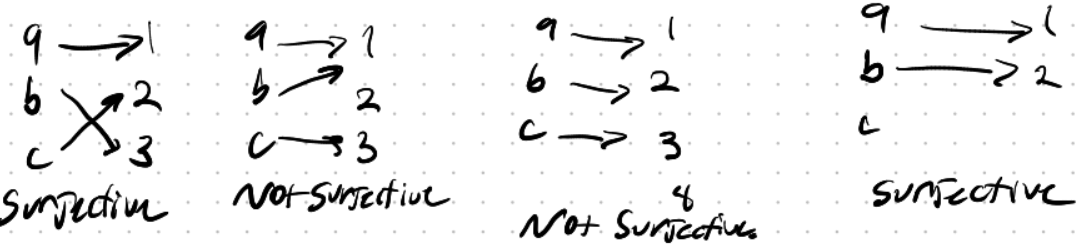
\includegraphics[width=0.8\linewidth]{surjective.png}
        \end{figure}

        \begin{mdframed}
            \textbf{Ex. } $f: \mathbb{R}\times \mathbb{R} \rightarrow \mathbb{R}\times \mathbb{R}, f(x,y) = (2x,y)$. Show that $f$ is surjective. 

            Take $(a,b) \in \mathbb{R}\times\mathbb{R}$ in the codomain and find $(x,y)\in\mathbb{R}\times\mathbb{R}$ in the domain such that $f(x,y)=(a,b)$.
            \begin{align*}
                (2x,y) = (a,b) \implies 2x = a \implies x= \frac{a}{2} \text{ and } y=b
            \end{align*}
            So for all $(a,b)\in \mathbb{R}\times \mathbb{R}, f(\frac{a}{2},b) = (a,b)$
        \end{mdframed}

        \subsection{Bijective Functions}
        A bijective function is a function that is both injective, and surjective. 

        \subsection{Composition of Functions}
        Let $f: A\to B$ and $g:B \to C$.
        
        The composition of $g$ and $f$, $g\circ f$, is the function from $A$ to $C$.
        \begin{align*}
            g\circ f(a) = g(f(a))
        \end{align*}
        \begin{figure}[H]
            \centering
            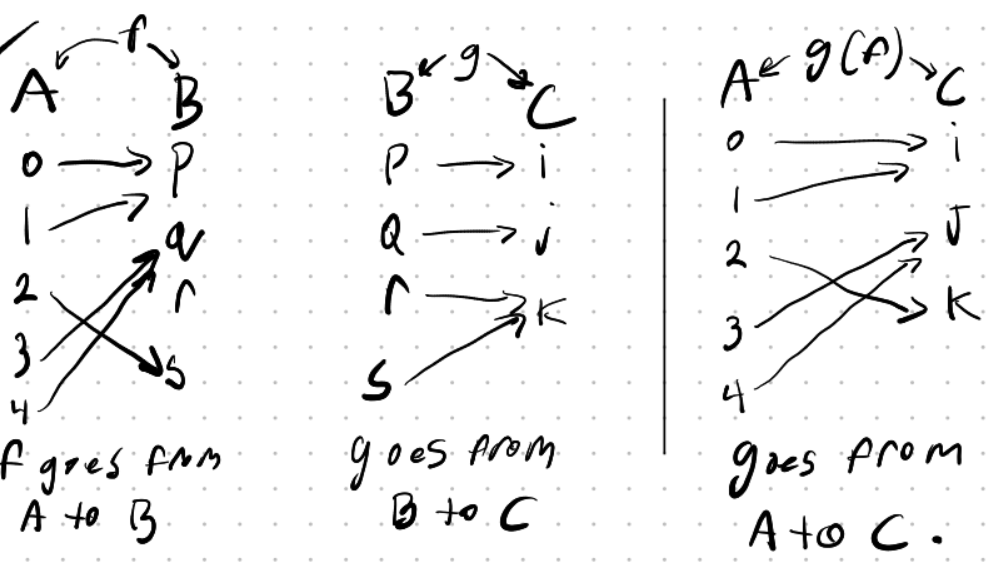
\includegraphics[width=0.6\linewidth]{composition-of-functions.png}
        \end{figure}

        \subsection{Identity Function}
        Let $A$ be a set. 
        
        The identity function on the set $A$ denoted $id_A$ is a function from $A$ to $A$.
        \begin{align*}
            id_A (x) = x \text{ } \forall \text{ } x\in A
        \end{align*}

        \subsection{Inverse of a Function}
        $f: A\to B$. The inverse of $f$, if it exists, is $f^{-1}: g\to A$ such that:
        \begin{align*}
            &f^{-1} \circ f = id_A &f\circ f^{-1} = id_B
        \end{align*}

        To find the inverse of a function with $x$ and $y$, we first let $x=y$ and $y=x$ and then solve for $y$ in terms of $x$.

        To verify that the found function is indeed an inverse, we then need to verify that both $f\circ f^{-1} (x) = x$, and $f^{-1} \circ f(x) = x$.

    \section{Counting}

        \subsection{Permutations}
        An $R$ permutation of a set is a way to order $R$ elements of a set. This is denoted by $P(n,R)$ which is the number of $R$ permutations of a set of $n$ elements.
        \begin{align*}
            P(n,r) = n(n-1)(n-2)...(n-r+1)
        \end{align*}

        \subsection{Combinations}
        Combinations are like permutations but for when order does not matter. 

        A permutation would count (1,2) and then (2,1) as different elements, while combinations would only count it once. 

        An r combination of a set of n elements is denoted as $C(n,r) = \frac{n!}{r!(n-r)!}$.
        
        \begin{mdframed}
            \textbf{Ex. } Passwords are composed of 4 letters and 3 digits in any order. How many passwords?

            First we need to choose the position of the 3 digits. Here order does not matter. If we choose positions (1,2,3) or (3,1,2), it does not matter. 

            ==$>$ $C(7,3)=35$

            Then we choose the 3 digits (10 options for each)

            ==$>$ $10\cdot 10\cdot 10$

            Finally we choose the 4 letters (26 letters for each)

            ==$>$ $26\cdot 26\cdot 26\cdot 26$

            The total is the product of all those. 

            ==$>$ $35\cdot 26^4 \cdot 10^3 = $CALC
        \end{mdframed}

        \begin{mdframed}
            \textbf{Ex. } We have 7 people A, B, C, D, E, F, G. We are taking a picture of 5 of them, but A and B must be adjacent. How many options are there if order \emph{does} matter?

            First we need to decide whether we want AB or BA. 

            ==$>$ 2 Options

            Then we need to decide where AB will go. Usually we would have 5 places, but since AB take up 2, we only actually have 4. 

            ==$>$ 4 options

            Finally, we need to choose the other 3 people from the 5 remaining people. Recall that order does matter. 

            ==$>$ $P(5,3) = 5\cdot 4\cdot 3 = 60$ options

            So the answer is $2\cdot 4\cdot 60 = 480$.
        \end{mdframed}

        \subsection{Permutations with Repetitions}
        Generally, the number of permutations of n objects containing $n_1$ indistinguishable objects of a first type, $n_2$ indistinguishable objects of a second type ... to $n_r$ indistinguishable objects of an nth type is: 
        \begin{align*}
            \frac{n!}{n_1!n_2!...n_r!}
        \end{align*}

        \begin{mdframed}
            \textbf{Ex. } How many permutations of the word "AAABBCD" do we have?
            \begin{align*}
                = \frac{\text{Total Permutations}}{\text{Number of B permutations }\cdot \text{Number of A permutations}} = \frac{7!}{3!\cdot2!}
            \end{align*}
        \end{mdframed}

        \subsection{Inclusion Exclusion Principle}
        This principle states:
        \begin{itemize}
            \item $|A\cup B| = |A| + |B| - |A\cap B|$
            \item $|\overline{A\cup B}|=|U| - |A\cup B|$
        \end{itemize}

        Recall that $U$ is the universal set (All the stuff we are considering at the moment).

        \begin{mdframed}
            \textbf{Ex. } How many 5 letter words start with A or end with ZZ?

            There are 2 ways to do this. 
            
            We can either count all the words that start with A, and then count all the words that end with ZZ, but then we would need to remove the ones that were double counted (ones that start with A AND end with ZZ)

            The other way would be to count the total words, and then remove all the words that we don't want (ones that do NOT start with A or end with ZZ)

            If we do it the first way, we get $26^4 + 26^3 - 26^2$ and if we do it the second we get $26^5 - (25\cdot26\cdot26\cdot(26^2-1))$. The reason the part for ZZ is weird, is because for those 2 letters there is only ONE option with ZZ. We do not care about ZA or CZ, only ZZ. So there are $26^2-1$ options for the last 2 letters.
        \end{mdframed}

    \section{Proof by Induction}
    Proof by induction works by proving 2 propositional statements of a proposition $P$ are true. 
    \begin{itemize}[noitemsep]
        \item $P(n_0)$ is true
        \item $P(n) \rightarrow P(n+1)$ is true $\forall \text{ } n\ge n_0$
    \end{itemize}
    If we can prove these 2 facts, then $P(n)$ is true $\forall \text{ } n\ge n_0$

        \subsection{Strong Induction}
        Strong induction is like regular induction except instead of just finding one base case, we will find multiple. 

        If we have 2 base cases, then in the induction step, we can use both n, and n+1. 

    \section{Binomial Theorem}
    Let $x,y$ be variables and let $n>0 \in \mathbb{Z}$.
    \begin{align*}
        (x+y)^n = \sum_{i=0} ^n C(n,i) \cdot x^{n-i} \cdot y^i
    \end{align*}

    \begin{mdframed}
        \textbf{Ex. } Determine the coefficient of $x^{12}y^{17}$ of $(3x^2-5y)^{23}$.

        If we use the binomial theorem, this is very easy.
        \begin{align*}
            (3x^2-5y)^{23} = \sum_{i=0}^{23} C(23,i)\cdot (3x^2)^{23-i}(5y)^i = \sum_{i=0}^{23} C(23,i)\cdot 3^{23-i}\cdot 5^i\cdot x^{46-2i}\cdot y^i
        \end{align*}
        Now we can find i using those 2 equations. $46-2i = 12 \text{ and } i = 17$.

        We get a value of 17 for i which we just sub into the equation.
        \begin{align*}
            = C(23,17)3^{23-17}(-5)^{17} = \text{CALC}
        \end{align*}
    \end{mdframed}
    
    \section{Combinatorial Proof}
    This type of proof involves solving a problem in 2 different ways, and if both give the same answer, then it is proven.

    Pascal's Identity is useful for combinatorial proofs. It states that if $n\ge k+1$, and $k\ge 0$, and $n,k \in \mathbb{Z}$, then:
    \begin{align*}
        C(n,k) + C(n,k+1) = C(n+1, k+1)
    \end{align*}

    \section{Pigeonhole Principle}
    If we have k+1 objects, and k boxes, then at least one box will have at least 2 objects.

    For these problems, we want to think of the worst case scenario, and then assign what is the objects, and what is the boxes, and then solve. 

    \begin{mdframed}
        \textbf{Ex. } Consider a standard deck of cards. How many cards must we draw to ensure we draw 2 cards of the same colour?

        We can assign boxes and objects. The boxes are the card colours (Red and Black).

        The objects are the cards. 

        Since there are 2 boxes, then we must draw 2+1 cards to ensure at least one of the boxes has 2 items.
    \end{mdframed}

    \section{Graph Theory}
    A graph $G$ contains Vertices denoted $V(G)$ and Edges denoted $E(G)$.

    A graph is called \emph{simple} if it has no loops, and no parallel edges. 

    2 vertices are called adjacent if there exists an edge that connects the 2 vertices. 

    The adjacency matrix of a graph shows how many edges go from each vertex to each other vertex. 

    An edge is called incident to all vertices that it is touching.

    \begin{mdframed}
        \textbf{Ex. } Find the adjacency matric for this graph:
        \begin{figure}[H]
            \centering
            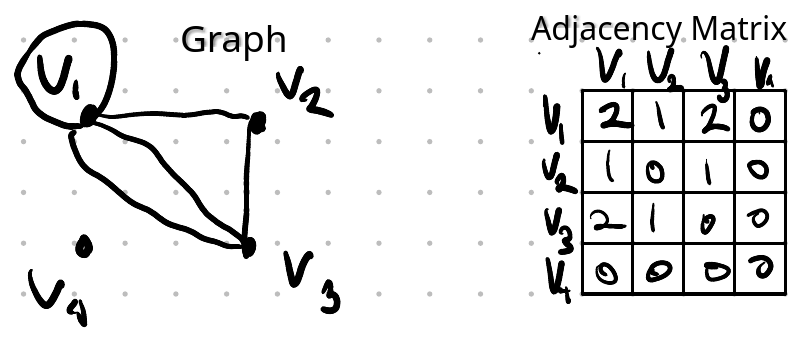
\includegraphics[width=0.5\linewidth]{Ex7.png}
        \end{figure}

        The matrix was created by seeing how many edges go from each vertex to each other vertex. Loops are counted twice.

    \end{mdframed}

        \subsection{Degree}
        The degree of a vertex $V$ of a graph $G$ denoted deg(V) is the number of edges incident to V where loops are counted twice. 

        The degree sequence of a graph with vertices $\{V_1, V_2, ..., V_n\}$ is $(deg(V_1), deg(V_2), ..., deg(V_n))$.

        \begin{mdframed}
            \textbf{Ex. } Find the degrees and degree sequence of this graph.
            \begin{figure}[H]
                \centering
                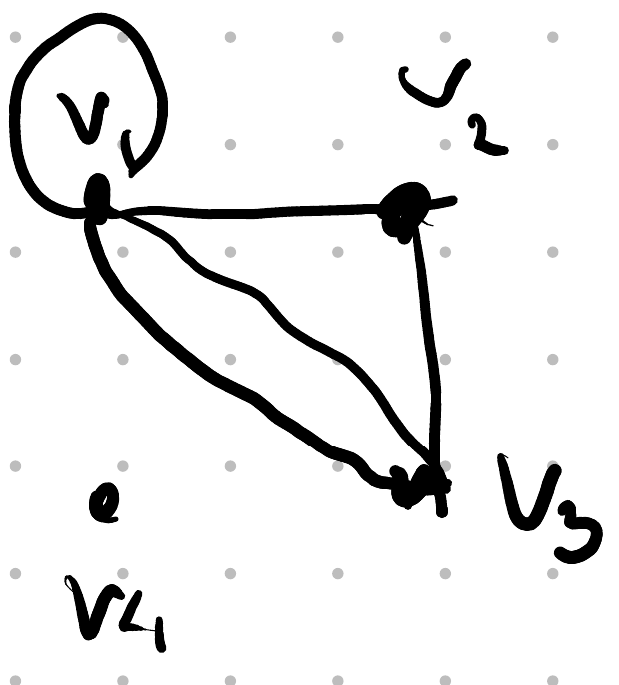
\includegraphics[width=0.15\linewidth]{ex8.png}
            \end{figure}

            I can simply count the number of edges coming out of each vertex. 

            $deg(V_1) = 5, deg(V_2) = 2, deg(V_3) = 3, deg(V_4) = 0$

            For the degree sequence, it is just the set of those degrees. Order does not matter.

            $(0,2,3,5)$

        \end{mdframed}

        \subsection{Handshake Lemma}
        This is a very simple statement that often comes in use. 
        \begin{align*}
            \sum_{V\in V(G)} deg(V) = 2|E(G)|
        \end{align*}

        \begin{mdframed}
            \textbf{Ex. } Does a graph exist with degree sequence (0,1,1,1)?

            No, according to the handshake lemma, the sum of degrees (3) must be half the number of edges. So there would be 1.5 edges which is not possible.
        \end{mdframed}

        \subsection{Isomorphism}
        An isomorphism from a graph G to another graph H is a bijective function $f:V(G)\rightarrow V(H)$ such that for all $u, v \ni V(G)$, $u$ is adjacent to $v$ iff $f(u)$ is adjacent to $f(v)$. If $f$ exists, then $G$ and $H$ are isomorphic. 

        \begin{mdframed}
            \textbf{Ex. } Show the following 2 graphs are isomorphic. 

            \begin{figure}[H]
                \centering
                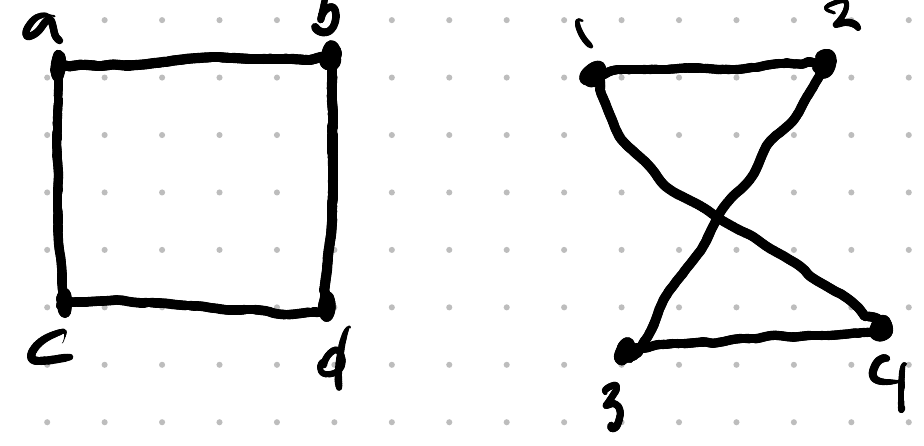
\includegraphics[width=0.3\linewidth]{ex9.png}
            \end{figure}

            We need to come up with a function $f$ that translates each vertex on the first graph (a,b,c,d) to each vertex on the second (1,2,3,4). This should basically make the first look like the second. 
            \begin{align*}
                & f(a) = 1 & f(b) = 2 \\
                & f(c) = 4 & f(d) = 3
            \end{align*}

            Now, we need to show that each adjacency in the first graph exists in the second graph. 

            Note: $A \sim B$ means $A$ is adjacent to $B$.
            \begin{align*}
                & a\sim b \leftrightarrow 1\sim 2 & b\sim d \leftrightarrow 2\sim 3\\
                & d\sim c \leftrightarrow 4\sim 3 & c\sim a \leftrightarrow 4\sim 1
            \end{align*}

            We see that all those are true, so these graphs are indeed isomorphic. 

        \end{mdframed}

        If we want to show 2 graphs are not isomorphic, we need to find a fundamental difference between them such as:
        \begin{itemize}[noitemsep]
            \item Difference in the number of edges
            \item Difference in the number of vertices
            \item Different degree sequence
            \item A subgraph of one graph that is not present in the other
        \end{itemize}

        \subsection{Subgraph}
        Let G and H be 2 graphs. We say H is a subgraph of G if $V(H)\subseteq V(G)$ and $E(H)\subseteq E(G)$.

        \subsection{Complete Graphs}
        Let $n \ge 0 \in \mathbb{Z}$. The complete graph on $n$ vertices denoted by $K_n$ has the following properties:
        \begin{itemize}[noitemsep]
            \item $K_n$ is simple
            \item The number of vertices in $K_n = n$
            \item Each pair of vertices is linked by \emph{exactly} 1 edge.
        \end{itemize}

        \begin{figure}[H]
            \centering
            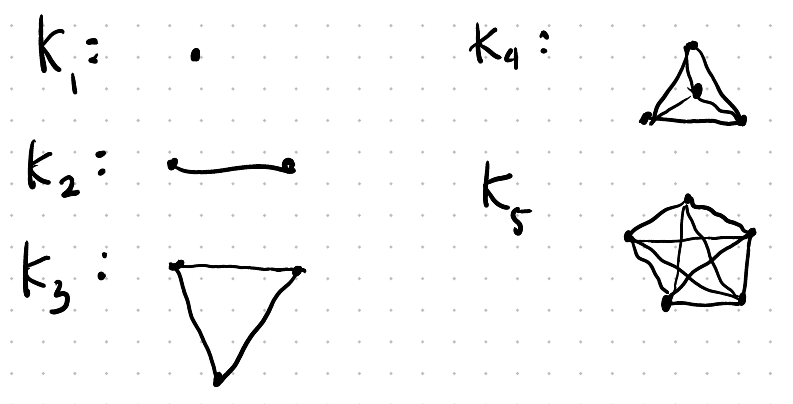
\includegraphics[width=0.5\linewidth]{kn.png}
        \end{figure}

        \subsection{Cycles}
        Let $n\ge 0 \in \mathbb{Z}$. A cycle of length $n$ denoted $C_n$ has the following properties:
        \begin{itemize}[noitemsep]
            \item $V(C_n) = \{u_1, u_2, u_3, ..., u_n\}$
            \item $u_1 \sim u_2, u_2 \sim u_3, ..., u_{n-1} \sim u_n, u_n \sim u_1$
        \end{itemize}

        \begin{figure}[H]
            \centering
            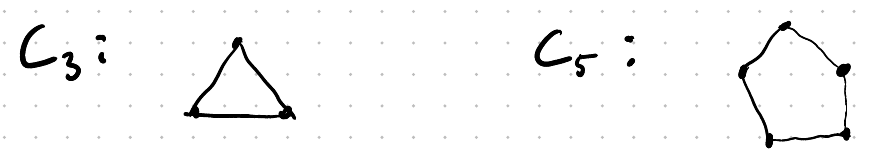
\includegraphics[width=0.5\linewidth]{cycle.png}
        \end{figure}

        \subsection{Bipartite Graphs}
        A graph is Bipartite if we can colour the vertices of G using 2 colours in such a way that no 2 adjacent vertices receive the same colour. 

        \subsection{Planar Graphs}
        A graph is planar if it can be drawn on a plane without intersecting edges. Such a drawing is called a planar embedding. 

        We can find out that a graph is not planar if $K_5$ of $K_3$ can be obtained from the original graph by deleting edges, or vertices. 

        We also have the following theorum about a simple connected planar graph. Let $v\in V(G), e\in E(G), $ and $f$ represent the number of faces of G. 
        \begin{align*}
            v-e+f=2
        \end{align*}

        \subsection{Chromatic Numbers}
        Let G be a graph. A colouring of G is a way of assigning a colour to every vertex such that adjacent vertices receive \emph{different colours}. The \emph{minimum} number of colours required to colour G is called the chromatic number of G denoted $\chi (G)$.

        We can come up with chromatic numbers easily for complete graphs and cycles. 
        \begin{itemize}[noitemsep]
            \item $\chi(K_n) = n$
            \item $\chi(C_n) = \{2 \text{ if n is odd }, 3 \text{ if n is even }, 0 \text{ if } n=1\}$.
        \end{itemize}

        \subsection{Chromatic Polynomial}
        The chromatic polynomial of a graph G is $P_G : \mathbb{N} \rightarrow \mathbb{N}$. $P_G (\lambda) = $ the number of ways to colour G using $\lambda$ colours. 

        We have the following formula with simple connected graphs to find the chromatic polynomial for G.
        \begin{align*}
            P_G (\lambda) = P_{G-e} (\lambda) - P_{G\backslash e} (\lambda)
        \end{align*}

        Note that $G-e$ means to delete an edge $e$, and $G\backslash e$ means to contract $e$. Contract means to remove the edge $e$, and then fuse together the ends of $e$.

        \begin{mdframed}
            \textbf{Ex. } Find the chromatic polynomial for G. 

            \begin{figure}[H]
                \centering
                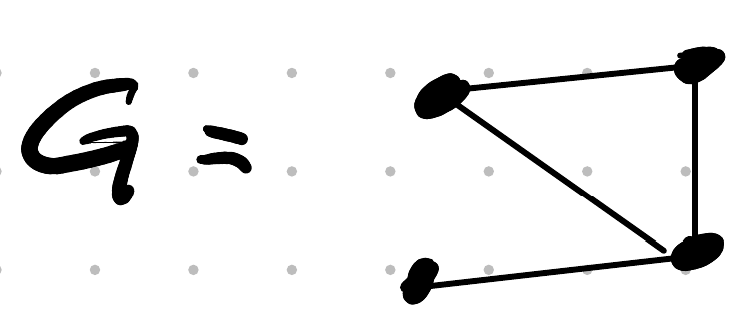
\includegraphics[width=0.2\linewidth]{ex10.png}
            \end{figure}

            We will use the formula. First we need to choose an edge to deal with. I will choose the middle edge, and then delete and contract it. 

            Note: The square brackets around the graph mean its chromatic polynomial. 

            \begin{figure}[H]
                \centering
                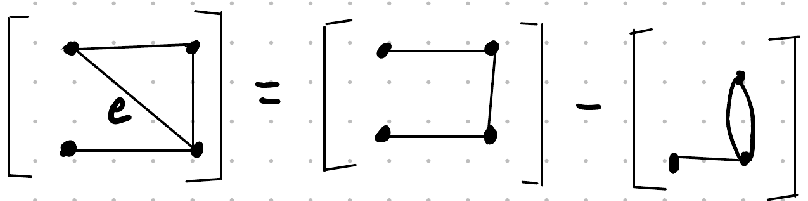
\includegraphics[width=0.4\linewidth]{ex10 2.png}
            \end{figure}

            Then we can replace the loop with just a line since chromatic numbers don't care about loops. 

            \begin{figure}[H]
                \centering
                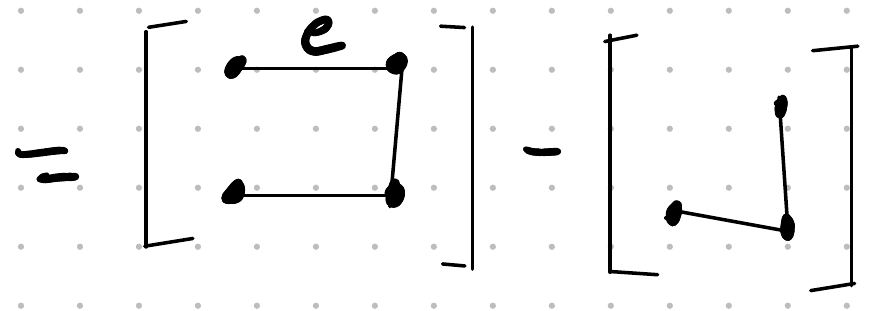
\includegraphics[width=0.3\linewidth]{ex10 3.png}
            \end{figure}

            Next, we can repeat the steps again. I will start with just the first graph above, and then simplify it. 

            \begin{figure}[H]
                \centering
                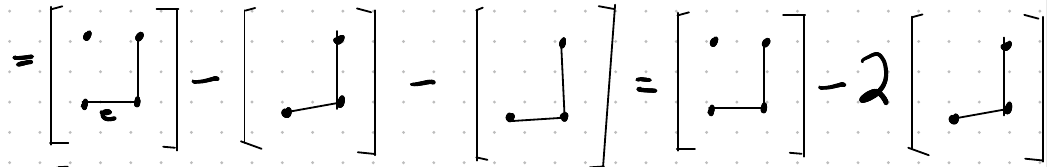
\includegraphics[width=0.8\linewidth]{ex10 4.png}
            \end{figure}

            Then I can repeat this over and over again following the formula until we are left with empty graphs.

            \begin{figure}[H]
                \centering
                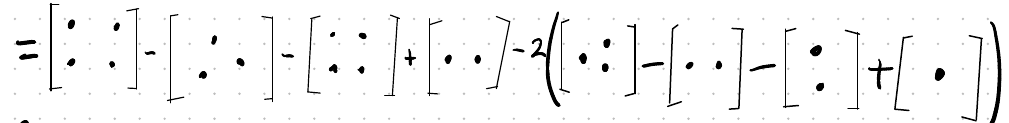
\includegraphics[width=0.9\linewidth]{ex10 5.png}
            \end{figure}

            We know the chromatic polynomial of an empty graph is related to its number of vertices, so we use that to solve.
            \begin{align*}
                P(\lambda) = \lambda^4-\lambda^3-\lambda^4+\lambda^2-2(\lambda^3-\lambda^2-\lambda^2+\lambda)
            \end{align*}
        \end{mdframed}

    \pagebreak
    \section{Appendix}
        \subsection{Propositional Logic Operators}
            \begin{centering}
                \textbf{Negation (not)}
                
                $\neg P $ means if P is true, then  $\neg P$  is False.
        
                \vspace{6pt}
                \begin{tabular}{c|c}
                    \textbf{$P$} & \textbf{$\neg P$} \\
                    \hline
                    T & F \\
                    F & T \\
                \end{tabular}
        
                \textbf{Conjunction (and)}

                $P \land Q $ is true if both P and Q are true.
                
                \vspace{6pt}
                \begin{tabular}{c c|c}
                    \textbf{$P$} & \textbf{$Q$} & \textbf{$P \land Q$} \\
                    \hline
                    T & T & T \\
                    T & F & F \\
                    F & T & F \\
                    F & F & F \\
                \end{tabular}
        
                \textbf{Disjunction (or)}

                $P \lor Q $ is true if at least one of P or Q is true.
                
                \vspace{6pt}
                \begin{tabular}{c c|c}
                    \textbf{$P$} & \textbf{$Q$} & \textbf{$P \lor Q$} \\
                    \hline
                    T & T & T \\
                    T & F & T \\
                    F & T & T \\
                    F & F & F \\
                \end{tabular}
        
                \textbf{Exclusive Or}

                $P \oplus Q $ is true if \emph{exactly} one of P or Q is true.
                
                \vspace{6pt}
                \begin{tabular}{c c|c}
                    \textbf{$P$} & \textbf{$Q$} & \textbf{$P \oplus Q$} \\
                    \hline
                    T & T & F \\
                    T & F & T \\
                    F & T & T \\
                    F & F & F \\
                \end{tabular}
        
                \textbf{Implication}

                $P \to Q $ is true if P implies Q. This means that if P is true, then Q \emph{must be} true as well.
                
                \vspace{6pt}
                \begin{tabular}{c c|c}
                    \textbf{$P$} & \textbf{$Q$} & \textbf{$P \to Q$} \\
                    \hline
                    T & T & T \\
                    T & F & F \\
                    F & T & T \\
                    F & F & T \\
                \end{tabular}
        
                \textbf{Biconditional Statement (iff)}

                $P \leftrightarrow Q $ is true \emph{if and only if} P is logically equivalent to Q. (They have the same values)
                
                \vspace{6pt}
                \begin{tabular}{c c|c}
                    \textbf{$P$} & \textbf{$Q$} & \textbf{$P \leftrightarrow Q$} \\
                    \hline
                    T & T & T \\
                    T & F & F \\
                    F & T & F \\
                    F & F & T \\
                \end{tabular}

            \end{centering}


        \subsection{Table of Laws of Logic}

        Let P, Q, and R be propositions, T and F represent True and False. 

        \begin{align*}
            1.& \indent P \to Q \equiv \lnot P \lor Q \\
            2.& \indent P \leftrightarrow Q \equiv (P \land Q) \lor (\lnot P \land \lnot Q) \\
            3.& \indent P \leftrightarrow Q \equiv (P\to Q) \land (Q\to P) \\
            4. &\indent P\lor \lnot P \equiv T\\
            5. &\indent P \land \lnot P \equiv F\\
            6. &\indent P \lor F \equiv P\\
            7. &\indent P \land T \equiv P \\
            8. &\indent P \lor T \equiv T \\
            9. &\indent P \land F \equiv F  \\
            10. &\indent P \lor P \equiv P \\
            11. &\indent P \land P \equiv P \\
            12. &\indent \lnot \lnot P \equiv P \\
            13. &\indent P \lor Q \equiv Q \lor P \\
            14. &\indent P \land P \equiv Q \land P \\
            15. &\indent (P \lor Q) \lor R \equiv P \lor (Q \lor R) \\
            16. &\indent (P \land Q) \land R \equiv P \land (Q \land R) \\
            17. &\indent P \lor (Q \land R) \equiv (P \lor Q) \land (P \lor R) \\
            18. &\indent P \land (Q \lor R) \equiv (P \land Q) \lor (P \land R) \\
            19. &\indent \lnot (P \land Q) \equiv \lnot P \lor \lnot Q \\
            20. &\indent \lnot (P \lor Q) \equiv \lnot P \land \lnot Q \\
            21. &\indent P \lor (P \land Q) \equiv P \\
            22. &\indent P \land (P \lor Q) \equiv P \\
            23. &\indent P \oplus Q \equiv (P \land \lnot Q) \lor (\lnot P \land Q) \\
        \end{align*}

        \subsection{Arguments Example}
        Here is a big example for arguments. 

        \begin{figure}[H]
            \centering
            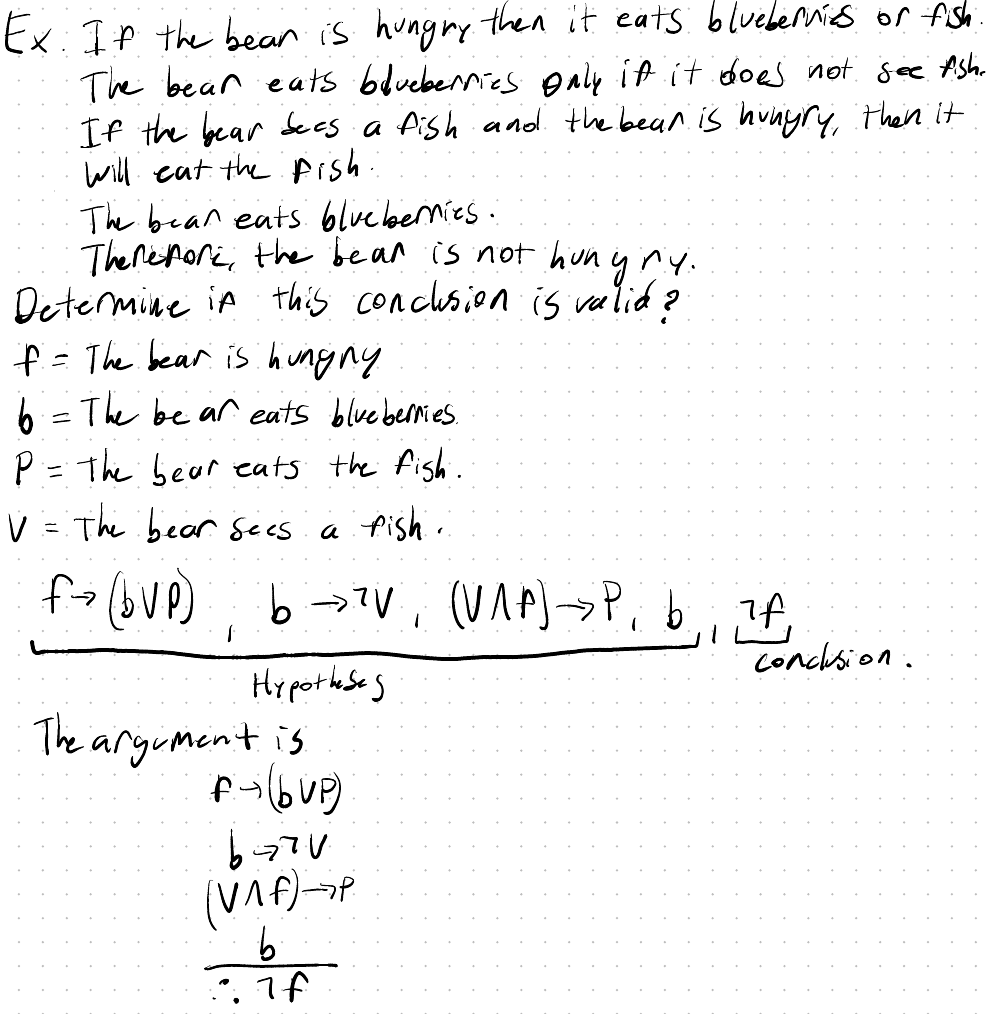
\includegraphics[width=0.7\linewidth]{ex4 1.png}
            
        \end{figure}

        Now we have the argument. We use truth tree to check.

        Recall that when checking the arguments, we put all the arguments at the top, and then the \emph{negation of the conclusion} hence $f$ rather than $\lnot f$.

        \begin{figure}[H]
            \centering
            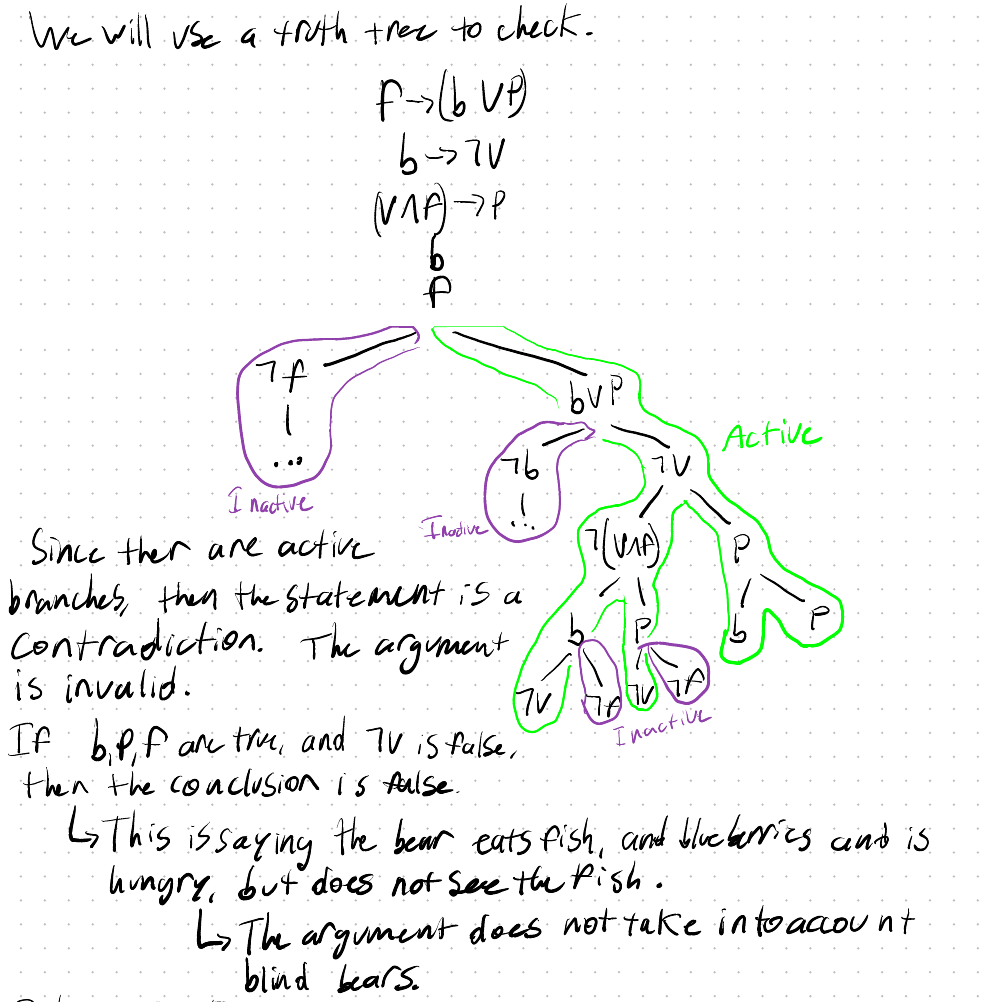
\includegraphics[width=0.7\linewidth]{ex4 2.png}
            
        \end{figure}

        As written in the picture, due to the active branch, there is a contradiction to the argument. This means that argument is invalid. There is a way to make it nonsensical by saying the bear eats fish, blueberries and is hungry however it does not see the fish. 
    
        
\end{document}